vocab-express is being implemented in node.js\footnote{\footnotesize \url{http://nodejs.org/}}, which is a platform built on V8\footnote{\footnotesize V8 is Google's open source JavaScript engine.} for easily building fast, scalable network applications. 
Figure \ref{fig:workflow} depicts the workflow of vocab-express. Next we describe the steps of the workflow

\begin{figure}[hbt!p]
\begin{center}
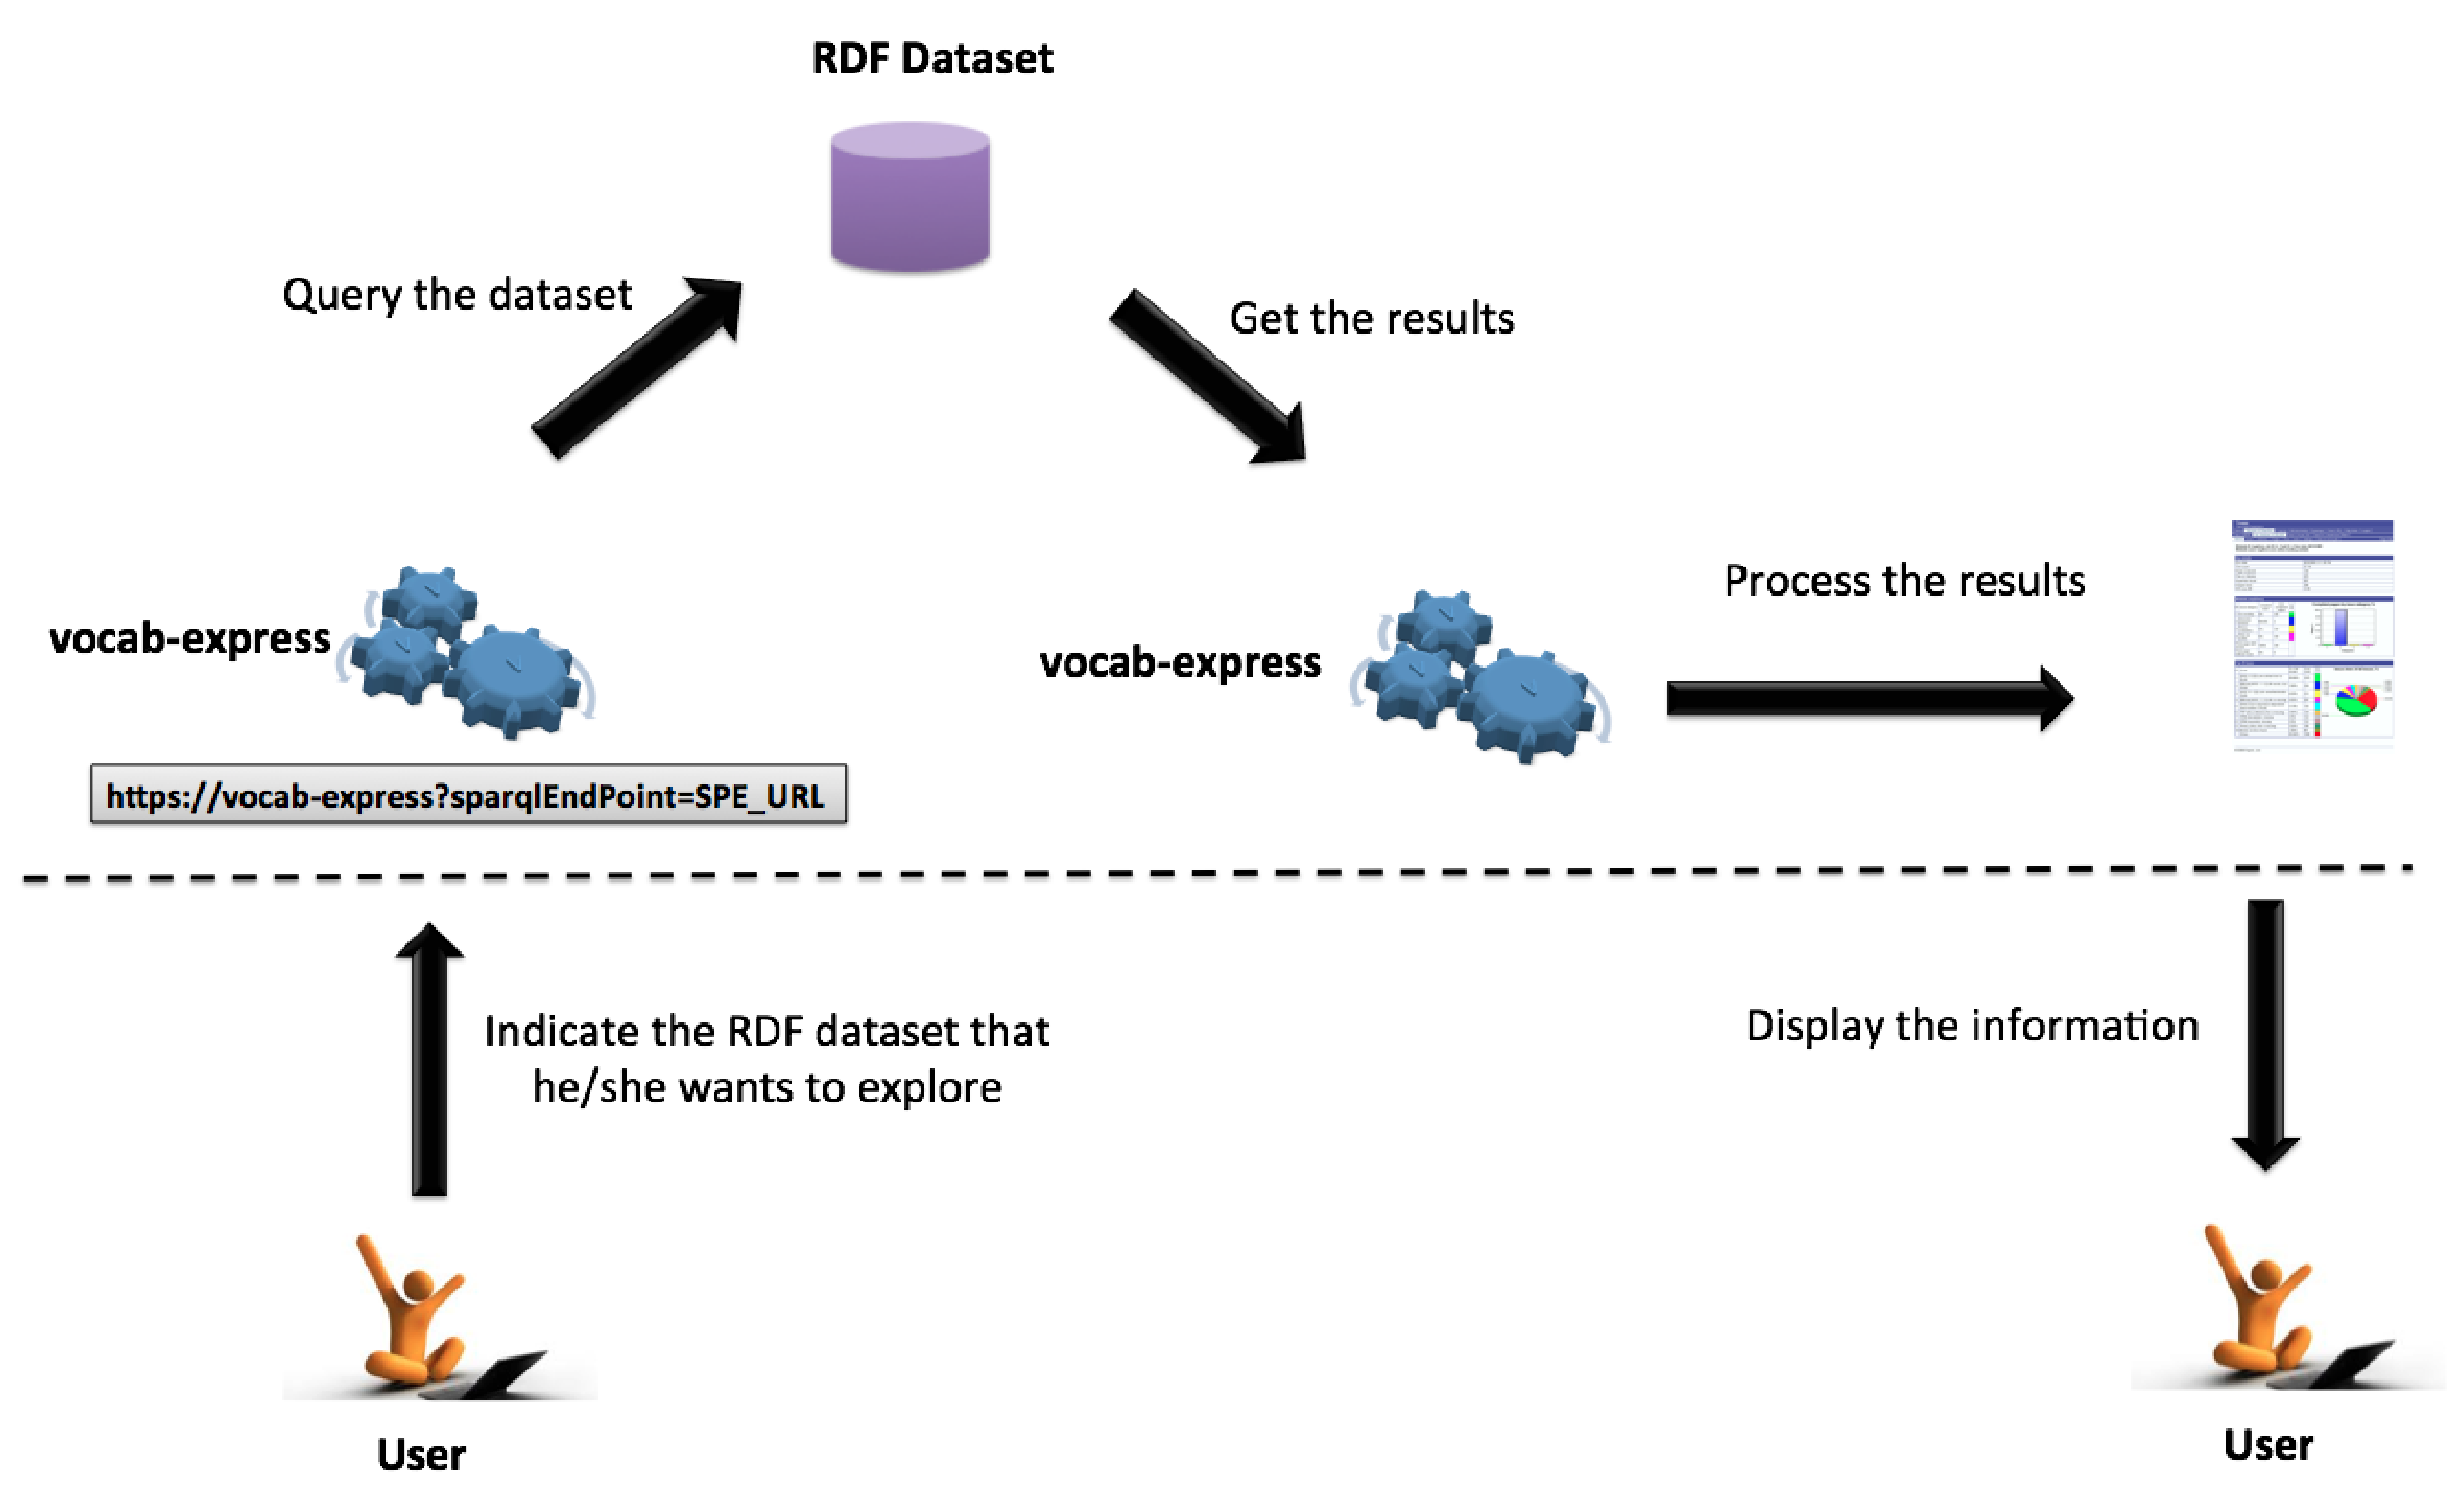
\includegraphics[scale=0.22]{img/workflow.eps}
\end{center}
\label{fig:workflow} 
\caption{vocab-express workflow}
\end{figure}


\begin{enumerate}
	\item The user indicates the RDF dataset he/she wants to explore by providing its SPARQL endpoint URL
	\item vocab-express receives and validates the SPARQL endpoint URL
	\item vocab-express queries the SPARQL endpoint and gets results in JSON\footnote{\footnotesize \url{http://www.json.org}} format
	\item vocab-express processes the results and displays the information to the user
\end{enumerate}
The workflow is similar if the user provides the URL of the VoID file instead of the SPARQL endpoint.